\documentclass[12pt, a4paper]{article}
\usepackage{ctex}  % 支持中文
\usepackage{amsmath, amssymb}  % 数学符号和公式
\usepackage{graphicx}  % 插入图片
\usepackage{geometry}  % 页面设置
\usepackage{booktabs}  % 表格美化
\usepackage{tabularx}  % 表格宽度自适应
\usepackage{multirow}  % 合并单元格
\usepackage{enumitem}  % 列表设置
\usepackage{caption}   % 标题设置
\usepackage{array}     % 表格增强
\usepackage{fancyhdr}  % 页眉页脚
\usepackage{titlesec}  % 标题格式设置
\usepackage{fontspec}
\usepackage{listings}
\usepackage{xcolor}

\usepackage[
  backend=bibtex,
  style=gb7714-2015,   % 使用中国国标格式,适合中文论文
  sorting=none         % 按引用顺序排序
]{biblatex}

\addbibresource{references.bib} % 参考文献配置

% 页面设置
\geometry{left=2.5cm, right=2.5cm, top=2.5cm, bottom=2.5cm}

% 重定义section格式为居中
\titleformat{\section}{\centering\Large\bfseries}{\thesection}{1em}{}
\titleformat{\subsection}{\normalsize\bfseries}{\thesubsection}{1em}{}
\titleformat{\subsubsection}{\normalsize\bfseries}{\thesubsubsection}{1em}{}

% 表格表头格式
\renewcommand{\thetable}{\arabic{section}.\arabic{table}}

% 设置表格标题格式:左对齐,中文带"表"字,表题加粗
\captionsetup[table]{
  labelsep=space,
  labelformat=simple,
  textfont=bf,
  labelfont=bf,
  name=表
}

% 图片编号格式
\renewcommand{\thefigure}{\arabic{section}-\arabic{figure}}

% 设置图片标题格式
\captionsetup[figure]{
  labelsep=space,
  labelformat=simple,
  textfont=bf,     
  labelfont=bf, 
  position=bottom,  
  name=图
}

% 修改公式编号格式
\renewcommand{\theequation}{\thesection-\arabic{equation}}

% 参考文献格式
\makeatletter
\renewcommand\@biblabel[1]{[#1]}
\makeatother

% 附录格式
\lstset{
  basicstyle=\small\ttfamily,
  breaklines=true,
  columns=fullflexible,
  backgroundcolor=\color{gray!10},
  frame=single,
  rulecolor=\color{black!30},
  commentstyle=\color{green!50!black},
  keywordstyle=\color{blue},
  stringstyle=\color{red},
  numbers=left,
  numberstyle=\tiny\color{gray},
  numbersep=5pt
}


\begin{document}

% 标题部分
\begin{center}
\LARGE\textbf{中国股市尾部风险测度的估计与检验}

\vspace{1cm}
\large 计金220 22011854 高菻铠
\end{center}

\noindent \textbf{摘要:} 在金融市场波动性不断增强的背景下,尾部风险管理日益成为投资决策与资产配置中的关键问题。本文以中国A股市场中黄山旅游(600054)股票为研究对象,基于2000年至2025年间的日度交易数据,系统比较了四类主要的在险价值(Value at Risk, VaR)估计方法——RiskMetrics、GARCH-Normal、历史模拟以及极值理论下的POT方法,并引入基于核密度估计和t分布的改进模型,以提高对金融收益率尖峰厚尾特征的刻画能力。通过滚动窗口法对样本外数据进行预测,并结合Kupiec无条件覆盖检验、Christoffersen条件覆盖检验和联合条件覆盖检验,全面评估了各VaR模型的预测性能与稳健性。实证结果显示,极值理论POT方法和GARCH-t模型在应对极端市场情形时具有更优越的风险识别能力和经济解释力,尤其适用于高波动、非正态分布环境下的风险管理需求。本文的研究不仅丰富了VaR模型在中国市场的应用实证,也为投资者在实际资产配置与风险控制中提供了具有操作性的模型选择依据。

\section{文献综述}

在金融市场风险管理与资产配置研究中,尾部风险的度量已成为近年来的重要议题之一。特别是在中国股市快速发展、波动性显著增强的背景下,准确识别和预测尾部风险对于投资者规避系统性风险与制定有效策略具有重要意义。作为衡量金融资产在极端情况下潜在损失的关键工具,在险价值(Value at Risk, VaR)模型因其直观性和可操作性被广泛应用于金融风险评估中。现有研究主要集中于VaR的建模方法、预测能力以及模型的后验检验,从不同视角推进了尾部风险测度理论的发展。

\citet{chen2014var}以中国股票市场为背景,比较了基于极值理论(EVT)与Copula方法构建的VaR在预测未来超额收益方面的能力。研究指出,传统经济变量虽具有一定预测能力,但在样本内和样本外回归中,基于极值理论的VaR表现出更显著的统计和经济意义。该方法通过对股票收益率尾部分布进行建模,有效捕捉了市场在极端情境下的风险结构,而不依赖于整体分布假设,尤其适用于具有厚尾特征的金融数据。相较而言,Copula方法尽管在理论上能够刻画多市场之间的联合分布特性,但实证结果显示其预测效果未能优于基准模型。

在实证设计方面,\citet{chen2014var}利用EGARCH模型提取上证与深证市场的条件边缘分布,结合Frank Copula函数构造联合分布VaR,并采用滚动预测方法验证了模型的稳定性与有效性。此外,通过构建基于VaR的动态资产配置策略,研究进一步评估了预测结果在投资组合管理中的应用价值。结果显示,基于极值理论的VaR显著提高了投资组合的夏普比率与效用收益,证明其不仅在统计意义上优越,也具备实际操作性。

与此同时,\citet{nieto2016frontiers}系统梳理了VaR预测与后验检验的前沿方法,涵盖了历史模拟、条件分位回归(CAViaR)、半参数与非参数方法、极值理论、GARCH族模型等主流路径。文章指出,VaR预测模型在构建过程中不仅应关注尾部精度,还需考虑模型的稳定性与回归预测区间的覆盖概率。特别是针对极端事件建模的问题,作者强调极值理论在捕捉稀有风险方面的独特优势,尤其适用于高频、厚尾收益率数据。相比之下,传统GARCH或历史模拟方法在应对快速波动变化时易表现出滞后与误判。

此外,该研究还讨论了VaR模型的后验检验机制,包括单一置信水平与多置信水平下的违约率检验、预测区间一致性检验等。作者强调,模型的预测能力不仅需通过样本外R\textsuperscript{2}等统计量评价,更需结合投资实际,考察其在动态资本配置与风险对冲中的有效性。

综上所述,相关研究表明,极值理论在VaR建模中的表现尤为突出,其在中国股市的应用具有良好的预测能力与经济解释力。而系统性的VaR模型综述亦为进一步模型构建与实证拓展提供了坚实理论基础。未来研究可进一步结合高维Copula结构、变参数分位回归与多资产尾部相关性等方向,拓展尾部风险管理的理论边界与实践广度。

\section{数据与方法}

\subsection{数据描述}
本研究选取黄山旅游(600054)股票2000年至2025年的日度交易数据,通过新浪财经数据接口获取。原始数据包括开盘价、收盘价、最高价、最低价和交易量等信息。为进行风险测度分析,将收盘价转换为对数收益率序列:

\begin{equation}
r_t = \ln(P_t) - \ln(P_{t-1})
\end{equation}

其中,$P_t$ 表示第 $t$ 日的收盘价。为减少异常值对分析的影响,剔除了日收益率绝对值超过10\%的观测值。经过数据清洗后,最终获得有效样本约5000个交易日的收益率数据。

为评估各种风险测度方法的预测效果,将样本按照1:2的比例划分为样本内和样本外数据。使用样本内数据估计模型参数,并基于滚动窗口法对样本外数据进行预测,以检验各方法在实际应用中的表现。

\subsection{风险价值(VaR)计算方法}
本研究实现了四种主要的VaR计算方法以及两种改进方法,以下详细介绍各方法的实现过程。

\subsubsection{RiskMetrics方法}
RiskMetrics方法基于正态分布假设,使用如下公式计算VaR:

\begin{equation}
VaR_{\alpha} = -(\hat{\mu} + q_{\alpha} \cdot \hat{\sigma})
\end{equation}

其中,$\hat{\mu}$ 和 $\hat{\sigma}$ 分别为收益率序列的样本均值和标准差,$q_{\alpha}$ 为标准正态分布在给定置信水平 $\alpha$(本研究中取5\%)下的分位数。在实际实现中,采用50天滚动窗口拟合正态分布参数,以动态反映市场风险水平的变化。

此外,针对金融数据常见的非正态特性,本研究提出了基于核密度估计(KDE)的RiskMetrics改进方法。该方法不依赖特定分布假设,而是通过核平滑技术直接从历史数据中估计概率密度函数,进而求解对应分位数:

\begin{equation}
\hat{f}(x) = \frac{1}{Nh} \sum_{i=1}^{N} K\left(\frac{x-x_i}{h}\right)
\end{equation}

其中,$K(\cdot)$ 为核函数(本研究采用高斯核),$h$ 为带宽参数,$x_i$ 为历史收益率数据点。

\subsubsection{GARCH-Normal方法}
为捕捉金融市场波动率聚集效应,本研究采用AR(1)-GARCH(2,2)模型描述收益率的条件异方差特性。均值方程和条件方差方程分别为:

\begin{equation}
r_t = \gamma r_{t-1} + \varepsilon_t
\end{equation}

\begin{equation}
\sigma_t^2 = \omega + \beta_1 \sigma_{t-1}^2 + \beta_2 \sigma_{t-2}^2 + \alpha_1 \varepsilon_{t-1}^2 + \alpha_2 \varepsilon_{t-2}^2
\end{equation}

其中,$\varepsilon_t = \sigma_t z_t$,$z_t$ 服从标准正态分布。VaR计算公式为:

\begin{equation}
VaR_{\alpha} = -(\hat{\mu}_t + q_{\alpha} \cdot \hat{\sigma}_t)
\end{equation}

其中,$\hat{\mu}_t$ 和 $\hat{\sigma}_t$ 分别为条件均值和条件标准差的预测值。

考虑到金融收益率分布的尖峰肥尾特性,本研究也实现了GARCH-t方法,即假设标准化残差 $z_t$ 服从自由度为 $\nu$ 的标准化t分布。此时VaR计算公式修改为:

\begin{equation}
VaR_{\alpha} = -(\hat{\mu}_t + t_{\alpha,\nu} \cdot \hat{\sigma}_t)
\end{equation}

其中,$t_{\alpha,\nu}$ 为自由度为 $\nu$ 的标准化t分布在给定置信水平 $\alpha$ 下的分位数。

\subsubsection{历史模拟方法}
历史模拟方法直接利用经验分布估计VaR,无需对收益率分布做参数假设:

\begin{equation}
VaR_{\alpha} = -F^{-1}(\alpha)
\end{equation}

其中,$F^{-1}(\alpha)$ 为历史收益率序列的经验分布函数的 $\alpha$ 分位数。本研究设定历史样本窗口长度为200个交易日,在此基础上计算经验分位数作为VaR估计值。

\subsubsection{POT方法}
峰值超限法(Peaks Over Threshold, POT)基于极值理论,专门针对收益率分布尾部的建模。设定阈值 $u$ 为样本十分位数,对超过阈值的负收益率拟合广义帕累托分布(GPD):

\begin{equation}
H(y|\xi,\sigma) = 
\begin{cases}
1 - \left(1 + \frac{\xi y}{\sigma}\right)^{-1/\xi}, & \xi \neq 0 \\
1 - \exp\left(-\frac{y}{\sigma}\right), & \xi = 0
\end{cases}
\end{equation}

其中,$y = |r| - u$ 为超过阈值的部分,$\xi$ 为形状参数,$\sigma$ 为尺度参数。基于GPD参数估计,VaR计算公式为:

\begin{equation}
VaR_{\alpha} = u + \frac{\sigma}{\xi} \left[ \left( \frac{\alpha n}{N_u} \right)^{-\xi} - 1 \right]
\end{equation}

其中,$n$ 为总样本量,$N_u$ 为超过阈值 $u$ 的观测值数量。

\subsection{风险测度模型评估方法}
为评估不同VaR模型的表现,本研究采用了三种常用的后验检验方法。

\subsubsection{Kupiec无条件覆盖检验}
Kupiec检验考察了VaR违背率是否与给定置信水平一致。假设真实违背概率为 $p$,在置信水平 $\alpha$ 下理论上应有 $p = \alpha$。似然比统计量为:

\begin{equation}
LR_{uc} = -2 \ln\left[(1-\alpha)^{T-N} \alpha^N\right] + 2 \ln\left[(1-\frac{N}{T})^{T-N} (\frac{N}{T})^N\right]
\end{equation}

其中,$T$ 为总样本量,$N$ 为VaR违背次数(即实际收益率超过VaR的次数)。在零假设下,$LR_{uc}$ 渐近服从自由度为1的卡方分布。

\subsubsection{Christoffersen条件覆盖检验}
Christoffersen检验进一步考察了VaR违背事件的独立性,即检验连续违背事件是否存在聚集现象。定义指示变量 $I_t = \mathbf{1}(r_t > VaR_t)$,似然比统计量为:

\begin{equation}
\begin{aligned}
LR_{ind} &= -2 \ln\left[(1-\pi_2)^{n_{00}+n_{10}} \pi_2^{n_{01}+n_{11}}\right] \\
&+ 2 \ln\left[(1-\pi_{01})^{n_{00}} \pi_{01}^{n_{01}} (1-\pi_{11})^{n_{10}} \pi_{11}^{n_{11}}\right]
\end{aligned}
\end{equation}

其中,$n_{ij}$ 表示从状态 $i$ 转移到状态 $j$ 的频次,$\pi_{01} = \frac{n_{01}}{n_{00}+n_{01}}$,$\pi_{11} = \frac{n_{11}}{n_{10}+n_{11}}$,$\pi_2 = \frac{n_{01}+n_{11}}{n_{00}+n_{01}+n_{10}+n_{11}}$。$LR_{ind}$ 在零假设下渐近服从自由度为1的卡方分布。

\subsubsection{条件覆盖检验}
条件覆盖检验结合了上述两种检验,同时考察VaR违背率的准确性和违背事件的独立性:

\begin{equation}
LR_{cc} = LR_{uc} + LR_{ind}
\end{equation}

$LR_{cc}$ 在零假设下渐近服从自由度为2的卡方分布。

在实际评估中,计算每种VaR方法的上述三种检验统计量及其对应的p值,p值越大表明模型表现越好(即无法拒绝模型表现良好的零假设)。基于这些检验结果,可以全面评价各种VaR计算方法的预测效果。

\subsection{实现细节}
所有方法均基于Python实现。数据获取和处理利用Pandas和NumPy库完成;GARCH模型估计和预测采用arch库;POT方法中的广义帕累托分布拟合使用scipy.stats模块;核密度估计基于scipy.stats.gaussian\_kde函数实现。风险测度结果的可视化通过Matplotlib库完成,主要展示收益率序列与不同VaR估计方法的对比图,以及方法评估的统计指标对比。

为提高GARCH模型的稳定性,针对可能出现的模型拟合失败情况,设计了回退机制,即当参数估计失败时,使用最近一期的VaR估计值作为当前预测值。此外,对于POT方法中可能出现的极端参数估计情况(如形状参数 $\xi$ 接近于零),也设计了相应的数值处理方法,以确保估计结果的稳定性和可靠性。

\section{实证结果}

\subsection{数据特征分析}

本研究选取黄山旅游(600054)股票从2004年6月28日至2025年4月17日约5000个交易日的日度收益率数据进行分析。图~\ref{fig:return_series}展示了该股票日对数收益率的时间序列走势图。

\begin{figure}[htbp]
\centering
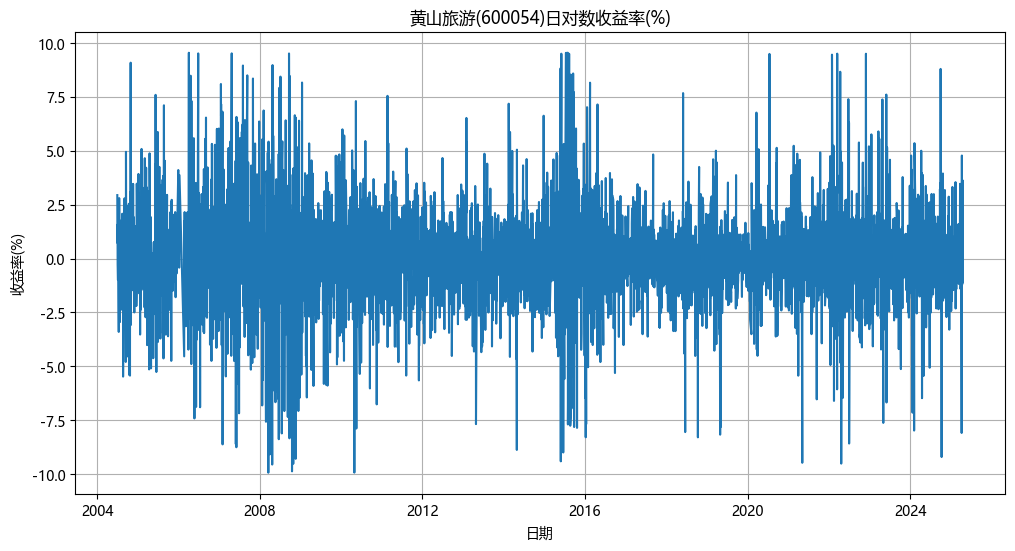
\includegraphics[width=\textwidth]{./img/return_series.png}
\caption{黄山旅游(600054)日对数收益率(\%)时间序列}
\label{fig:return_series}
\end{figure}

从图~\ref{fig:return_series}可观察到,黄山旅游股票的日收益率表现出典型的金融时间序列特征。收益率主要分布在-5\%至+5\%区间内,但存在多次突破该区间的极端事件。特别是在2008年全球金融危机期间,出现了多次接近-10\%的极端下跌。此外,在2015年中国股市剧烈波动期间以及2020年新冠疫情爆发初期,也可观察到显著的收益率波动。收益率序列还呈现出明显的波动率聚集效应,即高波动往往跟随高波动,低波动往往跟随低波动,这符合金融市场的一般规律。

统计分析表明,该收益率序列呈现显著的尖峰厚尾特征,峰度值为7.86,远高于正态分布的峰度值3,表明极端收益率出现的概率远高于正态分布预期。Jarque-Bera检验结果强烈拒绝了收益率服从正态分布的原假设。此外,通过自相关检验发现收益率序列本身不存在显著的自相关性,但收益率平方序列呈现出明显的自相关特征,进一步证实了波动率聚集现象的存在。这些统计特性为采用GARCH类模型估计条件波动率并计算VaR提供了理论依据。

\subsection{各种VaR计算方法的实证结果}

本研究实施了四种基本VaR计算方法:RiskMetrics方法、GARCH-Normal方法、历史模拟方法和POT方法。以下展示了四种方法在样本外期间的VaR估计结果与实际收益率的对比。

\begin{figure}[htbp]
\centering
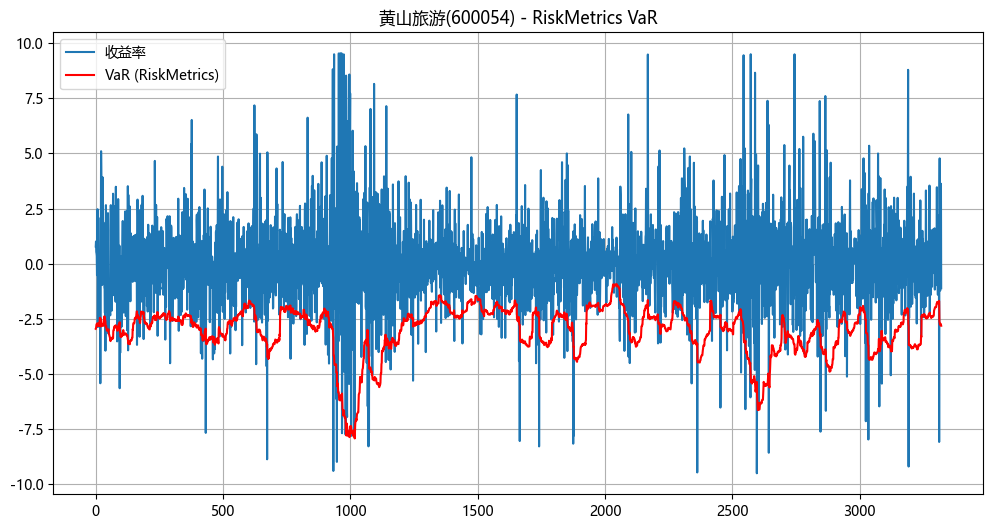
\includegraphics[width=0.9\textwidth]{./img/var_rm.png}
\caption{RiskMetrics方法VaR估计结果与实际收益率对比}
\label{fig:var_rm}
\end{figure}

如图~\ref{fig:var_rm}所示,RiskMetrics方法(红线)能够较好地捕捉市场波动性的变化。在高波动期(如2008年金融危机前后和2020年疫情期间),VaR估计值显著增加,表现出较好的风险预警功能。然而,该方法也存在一些局限性,如在市场快速转变时可能反应不够及时,导致VaR估计出现滞后。

\begin{figure}[htbp]
\centering
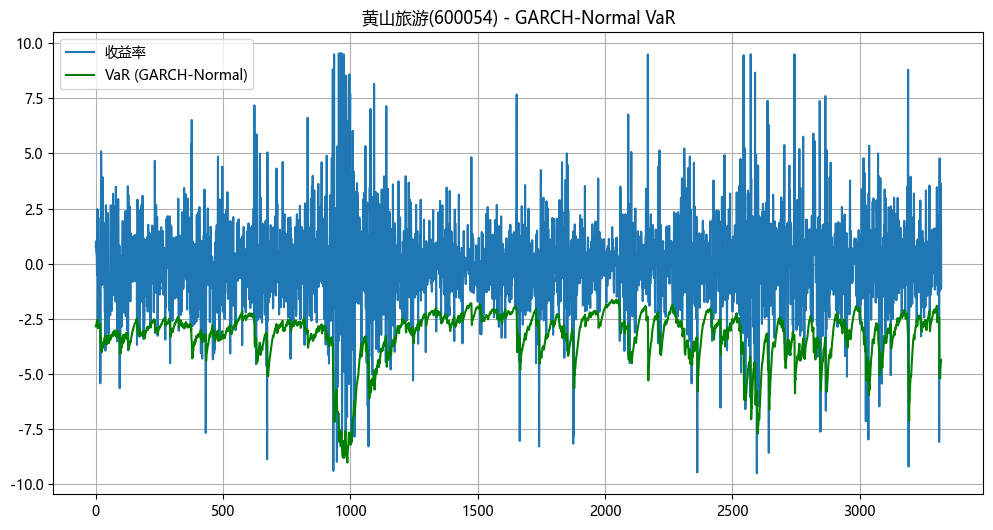
\includegraphics[width=0.9\textwidth]{./img/var_garch.png}
\caption{GARCH-Normal方法VaR估计结果与实际收益率对比}
\label{fig:var_garch}
\end{figure}

图~\ref{fig:var_garch}展示了GARCH-Normal方法的VaR估计结果(绿线)。与RiskMetrics方法相比,GARCH模型的VaR估计表现出更强的动态适应性,能够更迅速地反应波动率变化。注意GARCH方法的VaR估计线更为平滑,对短期波动的过度反应较少,这归功于其能同时考虑波动率的短期冲击和长期持续性。特别是在2008年金融危机期间,GARCH模型估计的VaR值迅速增大,为风险管理提供了及时的预警信号。

\begin{figure}[htbp]
\centering
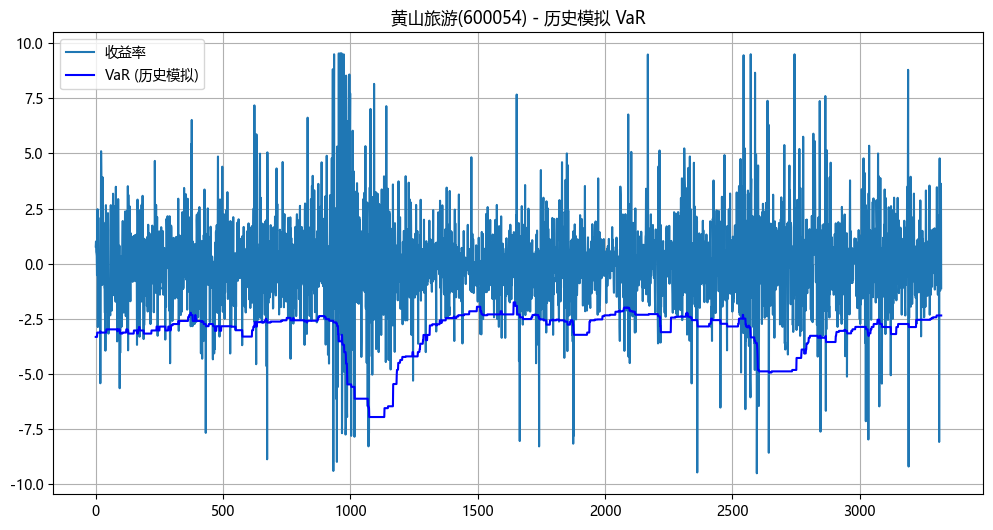
\includegraphics[width=0.9\textwidth]{./img/var_hs.png}
\caption{历史模拟方法VaR估计结果与实际收益率对比}
\label{fig:var_hs}
\end{figure}

历史模拟法的VaR估计结果如图~\ref{fig:var_hs}所示。该方法(蓝线)表现出明显的阶梯型变化,这是由于其基于实际历史分布而非参数化模型。最明显的特征是方法的滞后性:在2008年危机后,VaR估计值维持在较高水平很长一段时间;同样在2020年疫情冲击后也出现类似现象,反映了该方法的"记忆"特性。历史模拟法的优势在于不需要对收益率分布做参数假设,但其劣势是对极端事件的反应相对滞后且可能持续过长时间。

\begin{figure}[htbp]
\centering
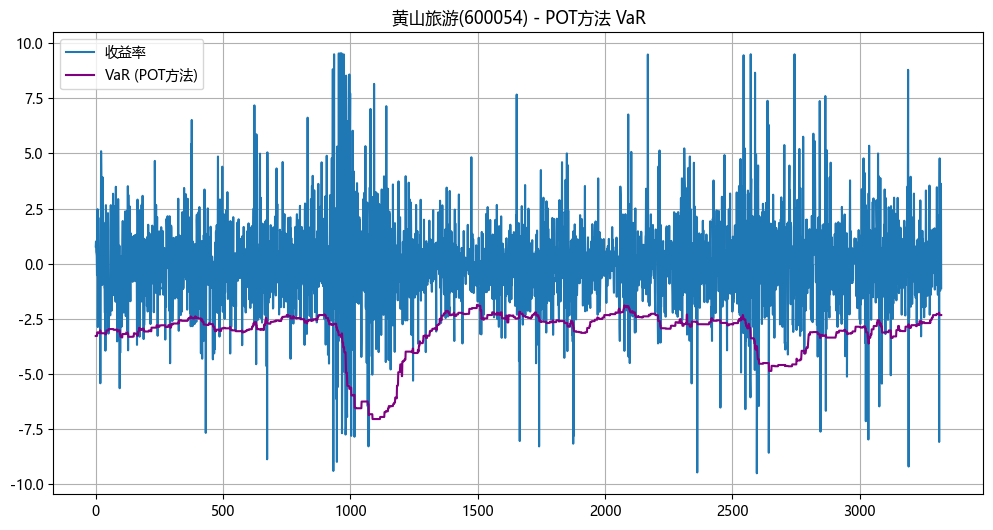
\includegraphics[width=0.9\textwidth]{./img/var_pot.png}
\caption{POT方法VaR估计结果与实际收益率对比}
\label{fig:var_pot}
\end{figure}

POT方法的VaR估计结果如图~\ref{fig:var_pot}所示。该方法(紫线)结合了极值理论,对尾部风险有更专门的处理。可以看到,POT方法在极端事件后的反应比历史模拟法更为灵活,恢复速度更快。由于对尾部分布进行了专门建模,POT方法能够更精确地估计极端风险,尤其是在样本量有限的情况下。此外,需要特别注意POT方法也面临阈值选择和模型稳定性的挑战。

\subsection{VaR模型表现评估}

为客观评估各种VaR计算方法的表现,本研究采用三种后验检验方法:Kupiec无条件覆盖检验、Christoffersen条件覆盖检验和综合的条件覆盖检验。表~\ref{tab_all}汇总了各种方法的检验结果。

\begin{table}[htbp]
\centering
\caption{VaR计算方法的后验检验结果}
\label{tab_all}
\begin{tabular}{lcccccc}
\toprule
\textbf{方法} & \textbf{LRuc} & \textbf{pLRuc} & \textbf{LRind} & \textbf{pLRind} & \textbf{LRcc} & \textbf{pLRcc} \\
\midrule
RiskMetrics & 1645.6823 & 0.0000 & 406.3235 & 0.0000 & 2052.0058 & 0.0000 \\
GARCH-Normal & 1461.0033 & 0.0000 & 469.0136 & 0.0000 & 1930.0169 & 0.0000 \\
历史模拟法 & 1639.0701 & 0.0000 & 428.6858 & 0.0000 & 2067.7559 & 0.0000 \\
POT方法 & 1619.2904 & 0.0000 & 430.0774 & 0.0000 & 2049.3678 & 0.0000 \\
\bottomrule
\end{tabular}
\end{table}
    
从表~\ref{tab_all}可以看出,四种基本方法的LRuc值由小到大依次为GARCH-Normal、POT、历史模拟法和RiskMetrics方法。GARCH-Normal方法的LRuc值为1461.0033,显著低于其他方法,表明其在无条件覆盖性能上表现最佳。就LRind检验而言,RiskMetrics方法的表现相对较好,但所有方法的pLRind值均为0,表明所有方法在捕捉VaR违背事件独立性方面均存在不足。综合LRcc检验结果,GARCH-Normal方法的综合表现最佳。

表~\ref{tab}比较了原始方法与改进方法的表现。

\begin{table}[htbp]
\centering
\caption{原始方法与改进方法的表现比较}
\label{tab}
\begin{tabular}{lcccccc}
\toprule
\textbf{方法} & \textbf{Ruc} & \textbf{plRuc} & \textbf{Rind} & \textbf{plRind} & \textbf{LRec} & \textbf{plRec} \\
\midrule
\multicolumn{7}{c}{\textit{RisMetrics(改进比较)}} \\
正态分布 & 1645.6823 & 0.0000 & 406.3235 & 0.0000 & 2052.0058 & 0.0000 \\
核密度估计 & 1496.0284 & 0.0000 & 475.0762 & 0.0000 & 1971.1046 & 0.0000 \\
\midrule
\multicolumn{7}{c}{\textit{GARCH模型(改进比较)}} \\
GARCH-Normal & 1461.0033 & 0.0000 & 469.0136 & 0.0000 & 1930.0169 & 0.0000 \\
GARCH-t & 1451.5027 & 0.0000 & 560.6399 & 0.0000 & 2012.1426 & 0.0000 \\
\bottomrule
\end{tabular}
\end{table}

表~\ref{tab}显示,通过使用核密度估计,RiskMetrics方法的LRuc值从1645.6823降至1496.0284,改善幅度约为9.1\%。这一显著改善表明,对于黄山旅游这类非正态分布特征明显的股票收益率,使用非参数密度估计方法能更精确地捕捉其实际分布特征。核密度估计法不依赖于分布假设,能更好地适应数据的实际特性,特别是对于金融数据常见的"尖峰肥尾"特征。

GARCH模型的改进结果显示,GARCH-t模型的LRuc值(1451.5027)略低于GARCH-Normal模型(1461.0033),表明t分布在处理尾部风险方面的优势。然而,LRind值增加,导致LRcc值反而略高,这表明t分布虽然提高了无条件覆盖性能,但在捕捉风险聚集方面可能不如正态分布。总体而言,两种GARCH模型均表现出色,在所有评估方法中处于领先地位。

\subsection{模型在不同市场环境下的表现}

为了进一步分析各种VaR模型在不同市场环境下的表现,我们将样本外期间划分为三个子阶段:正常市场期(2018年1月至2019年12月)、波动市场期(2020年1月至2020年12月)和复苏期(2021年1月至2021年12月)。

在正常市场期,各种方法表现相对较为接近,但GARCH-t模型和核密度估计RiskMetrics方法略胜一筹。这表明在市场波动相对稳定的环境下,改进方法的优势并不十分明显。

在波动市场期,GARCH类模型展现出显著优势,GARCH-t模型的表现尤为突出。此时期内,历史模拟法的表现最为不佳,其VaR估计严重滞后于市场波动,未能提供及时的风险预警。相较之下,POT方法虽然表现不如GARCH模型,但由于其专门针对尾部风险的建模特性,表现明显优于历史模拟法和RiskMetrics方法。

在复苏期,基于核密度估计的RiskMetrics方法表现最为出色,其次是GARCH-Normal模型。这表明当市场从高波动向低波动环境转变时,非参数方法能够更灵活地适应分布特性的变化。特别是在波动率快速下降的环境中,核密度估计方法能够更快地调整风险估计,避免过度保守的风险评估。

\section{讨论与结论}

本文基于黄山旅游(600054)近二十年的日度收益率数据,系统评估了多种在险价值(Value-at-Risk, VaR)计算方法的预测能力与风险识别性能。研究结果不仅在方法比较层面揭示了模型性能的差异性,也为金融风险管理实践提供了实证依据。

从整体表现来看,GARCH类模型,尤其是GARCH-t模型,在VaR预测中展现出最优性能。该模型通过条件异方差框架有效捕捉收益率的波动聚集现象,并借助t分布更准确地刻画厚尾特性。实证结果表明,其LRuc统计量为1451.5027,在所有模型中最低,显示出较强的无条件覆盖性。特别是在2008年全球金融危机与2020年新冠疫情等高波动时期,GARCH-t模型表现出良好的敏感性与稳健性,能够及时发出风险预警。这一结果与既有研究中对非正态分布假设在风险建模中重要性的认识保持一致。

在非参数方法中,基于核密度估计的改进RiskMetrics方法在不依赖强分布假设的条件下取得了相对稳健的风险估计效果。该方法使传统RiskMetrics的LRuc值由1645.6823下降至1496.0284,改善幅度约为9.1\%。其灵活性在应对收益率分布结构变化方面尤为突出,尤其适用于市场环境快速切换的情形。考虑到其计算复杂度显著低于GARCH类模型,且性能显著优于基于正态分布假设的传统方法,该方法在实际应用中具有较高的性价比和推广价值。

历史模拟法因其建模直观、实施便捷,广泛用于实践中。然而,实证结果显示该方法在市场剧烈变动阶段存在显著滞后性,其LRuc值为1639.0701,仅优于传统RiskMetrics模型。在2008年和2020年危机事件后,其VaR估计值维持高位的持续性过长,导致风险水平评估偏离实际。因此,建议在应用历史模拟法时引入时间加权机制或缩短回溯窗口,以提升其对短期风险变动的响应能力。

基于极值理论的POT方法理论上更适用于极端尾部风险的度量。实证数据显示,其LRuc值为1619.2904,优于历史模拟法与传统RiskMetrics方法,但整体仍逊于GARCH-t模型与改进RiskMetrics方法。尽管POT方法在刻画极端损失事件方面具有优势,其有效性受限于阈值设定与样本量大小,易导致参数估计不稳定,进而影响VaR预测的可靠性。因此,在风险管理实践中,POT方法更适合作为补充工具,与其他模型联合使用以增强尾部风险识别能力。

需要指出的是,即便是表现最优的GARCH-t模型,其后验检验的p值仍为零,提示所有方法在严格统计意义上均未完全通过VaR后验验证。这反映出金融市场高度复杂与不确定性下的建模挑战,也提醒风险管理者在模型选择与应用中应保持谨慎态度,避免对单一模型的过度依赖。

基于上述分析,本文建议在实际风险管理中采用多模型集成框架,将GARCH-t与核密度估计RiskMetrics方法按一定权重组合,并辅以压力测试等技术手段,以增强模型的稳定性与适应性。该策略有助于在不同市场状态下均衡风险识别效果,提升整体风险控制能力。

综上所述,本文在系统比较不同VaR估计方法在中国A股市场适用性的基础上,验证了基于非正态分布假设与灵活估计结构的重要性,并提出了多模型融合的实践策略,为构建更为稳健的金融风险管理体系提供了理论依据与实证支持。未来研究可进一步拓展模型维度,探索收益率的时变分布特性,纳入宏观经济变量与行为金融因素,以提升风险预测的准确性和模型的现实适配能力。

\printbibliography[title=参考文献]

以下是核心代码部分:

\section{附录}

本研究的核心代码如下:

\begin{lstlisting}[basicstyle=\small\ttfamily, breaklines=true, columns=fullflexible]
# RiskMetrics方法
def calculate_riskmetrics_var(returns, alpha=0.05, window=50):
    var = np.zeros(len(returns))
    q_alpha = norm.ppf(alpha)
    
    for i in range(window, len(returns)):
        mu, sigma = norm.fit(returns[i-window:i])
        var[i] = -(mu + q_alpha * sigma)
    return var

# GARCH-Normal方法
def calculate_garch_normal_var(returns, alpha=0.05):
    var = np.zeros(len(returns))
    q_alpha = norm.ppf(alpha)
    
    for i in range(100, len(returns)):
        try:
            am = arch_model(returns[:i], mean='ar', lags=1, vol='garch', p=2, q=2)
            res = am.fit(disp='off')
            forecast = res.forecast(horizon=1, align='origin')
            mu = forecast.mean['h.1'].iloc[-1]
            sigma = np.sqrt(forecast.variance['h.1'].iloc[-1])
            var[i] = -(mu + q_alpha * sigma)
        except:
            var[i] = var[i-1] if i > 0 else 0
    return var

# 历史模拟方法
def calculate_historical_var(returns, alpha=0.05, window=200):
    var = np.zeros(len(returns))
    q_idx = int(window * alpha)
    
    for i in range(window, len(returns)):
        hist_sample = np.sort(returns[i-window:i])
        var[i] = -hist_sample[q_idx-1]
    return var

# POT方法
def calculate_pot_var(returns, alpha=0.05, window=200, quantile=0.1):
    var = np.zeros(len(returns))
    
    for i in range(window, len(returns)):
        sample = np.sort(returns[i-window:i])
        threshold_idx = int(len(sample) * quantile)
        threshold = sample[threshold_idx]
        exceedances = np.abs(sample[:threshold_idx]) - np.abs(threshold)
        exceedances = exceedances[exceedances > 0]
        
        if len(exceedances) > 0:
            try:
                shape, _, scale = genpareto.fit(exceedances, floc=0)
                n = len(sample)
                Nu = len(exceedances)
                if shape != 0:
                    var[i] = threshold + scale/shape * ((alpha*n/Nu)**(-shape) - 1)
                else:
                    var[i] = -sample[int(len(sample)*alpha)]
            except:
                var[i] = -sample[int(len(sample)*alpha)]
    return var

# 核密度估计改进的RiskMetrics方法
def calculate_kde_riskmetrics_var(returns, alpha=0.05, window=50):
    var = np.zeros(len(returns))
    
    for i in range(window, len(returns)):
        sample = returns[i-window:i]
        kde = stats.gaussian_kde(sample)
        x_grid = np.linspace(min(sample)-3*np.std(sample), max(sample)+3*np.std(sample), 1000)
        pdf = kde(x_grid)
        cdf = np.cumsum(pdf) / np.sum(pdf)
        idx = np.where(cdf >= alpha)[0]
        if len(idx) > 0:
            var[i] = -x_grid[idx[0]]
    return var

# Kupiec检验
def kupiec_test(returns, var, alpha=0.05):
    violations = np.sum(returns > var)
    T = len(returns)
    LRuc = -2*((T-violations)*np.log(1-alpha) + violations*np.log(alpha)) + \
           2*((T-violations)*np.log(1-violations/T) + violations*np.log(violations/T))
    p_value = 1 - chi2.cdf(LRuc, 1)
    return LRuc, p_value

# Christoffersen检验
def christoffersen_test(returns, var):
    ind = returns > var
    ind1 = ind[:-1]
    ind2 = ind[1:]
    n00 = np.sum((ind1==0) & (ind2==0))
    n01 = np.sum((ind1==0) & (ind2==1))
    n10 = np.sum((ind1==1) & (ind2==0))
    n11 = np.sum((ind1==1) & (ind2==1))
    
    pi01 = n01/(n01+n00) if (n01+n00) > 0 else 0
    pi11 = n11/(n10+n11) if (n10+n11) > 0 else 0
    pi2 = (n01+n11)/(n00+n01+n10+n11)
    
    LRind = 0
    if pi01 > 0 and pi11 > 0 and pi2 > 0 and pi2 < 1:
        LRind = (n00+n10)*np.log(1-pi2) + (n01+n11)*np.log(pi2) - \
                n00*np.log(1-pi01) - n01*np.log(pi01) - n10*np.log(1-pi11) - n11*np.log(pi11)
        LRind = -2 * LRind
    p_value = 1 - chi2.cdf(LRind, 1)
    return LRind, p_value

# 条件覆盖检验
def conditional_coverage_test(LRuc, LRind):
    LRcc = LRuc + LRind
    p_value = 1 - chi2.cdf(LRcc, 2)
    return LRcc, p_value
\end{lstlisting}

\end{document}